\begin{frame}

\frametitle{Linker scripts}

\vspace{\fill}

How we normally think about compiling:
\begin{figure}
    \center
    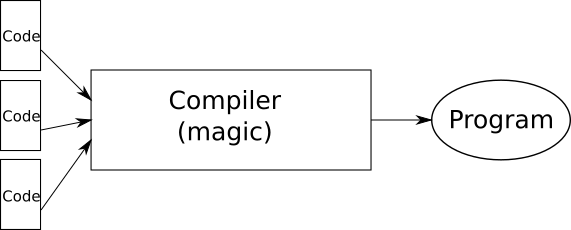
\includegraphics[width=0.8\textwidth]{figures/compiling_simple.png}
\end{figure}

\vspace{\fill}

\end{frame}


\begin{frame}

\frametitle{Linker scripts}

\vspace{\fill}

But we do actually have more control:
\begin{figure}
    \center
    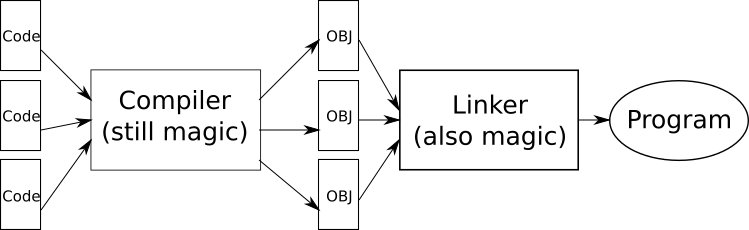
\includegraphics[width=0.8\textwidth]{figures/compiling.png}
\end{figure}

\vspace{\fill}

\end{frame}

\begin{frame}
\frametitle{Linker scripts}

\vspace{\fill}
An object file consist of:
\begin{itemize}
    \item Machine code (.text)
    \item Static data (.data)
    \item Information about uninitialized data (.bss)
    \item Symbols
    \item Other stuff (debugging information, compiler information, etc.)
\end{itemize}

\vspace{\fill}
We are interested in controlling how the object files are linked (merged) together.

\vspace{\fill}
\end{frame}

\begin{frame}
\frametitle{Linker scripts}

\vspace{\fill}
Most linker scripts includes:
\begin{itemize}
    \item ENTRY - Where is the entry point of the program?
    \item OUTPUT\_FORMAT - What should the format of the output be?
    \item SECTIONS - What is the layout of the output?
\end{itemize}

\end{frame}
\begin{frame}[fragile]
\frametitle{Linker script}
\vspace{\fill}
Example from KUDOS
\vspace{\fill}

\begin{lstlisting}
ENTRY(_start)
OUTPUT_FORMAT("elf64-x86-64")
phys = 0x00100000;
SECTIONS
{
    /*
     * Actual code
     */
    .text phys : AT(phys) {
        code = .;
        *(.boot*)
        *(.text*)
        *(.rodata*)
        . = ALIGN(4096);
    }
...
\end{lstlisting}

\vspace{\fill}

\end{frame}

\begin{frame}
    \frametitle{Linker script}
    \begin{center}
        WHO IS FIRST example
    \end{center}
\end{frame}
